

\tikzset{every picture/.style={line width=0.3pt}} %set default line width to 0.75pt        

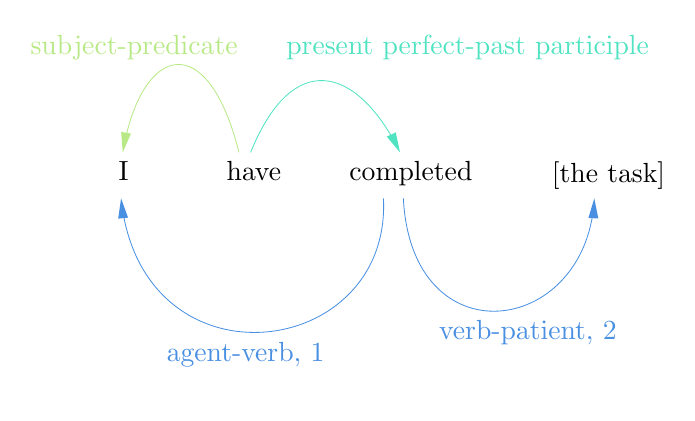
\begin{tikzpicture}[x=0.75pt,y=0.75pt,yscale=-0.8,xscale=0.8]
%uncomment if require: \path (0,300); %set diagram left start at 0, and has height of 300

%Curve Lines [id:da8298848597114246] 
\draw [color={rgb, 255:red, 74; green, 144; blue, 226 }  ,draw opacity=1 ]   (511.85,179.28) .. controls (505.89,260.1) and (401.95,273.83) .. (397,176.81) ;
\draw [shift={(512,176.81)}, rotate = 92.76] [fill={rgb, 255:red, 74; green, 144; blue, 226 }  ,fill opacity=1 ][line width=0.08]  [draw opacity=0] (12,-3) -- (0,0) -- (12,3) -- cycle    ;
%Curve Lines [id:da7977309817595222] 
\draw [color={rgb, 255:red, 74; green, 144; blue, 226 }  ,draw opacity=1 ]   (227.4,180.28) .. controls (242,293.42) and (389.95,273.83) .. (385,176.81) ;
\draw [shift={(227,176.81)}, rotate = 84.14] [fill={rgb, 255:red, 74; green, 144; blue, 226 }  ,fill opacity=1 ][line width=0.08]  [draw opacity=0] (12,-3) -- (0,0) -- (12,3) -- cycle    ;
%Curve Lines [id:da3756396013841674] 
\draw [color={rgb, 255:red, 80; green, 227; blue, 194 }  ,draw opacity=1 ]   (393.87,146.88) .. controls (368.83,97.77) and (330.61,86.11) .. (305,149.15) ;
\draw [shift={(395,149.15)}, rotate = 243.89] [fill={rgb, 255:red, 80; green, 227; blue, 194 }  ,fill opacity=1 ][line width=0.08]  [draw opacity=0] (12,-3) -- (0,0) -- (12,3) -- cycle    ;
%Curve Lines [id:da9846757481246158] 
\draw [color={rgb, 255:red, 184; green, 233; blue, 134 }  ,draw opacity=1 ]   (228.51,146.26) .. controls (240.2,83.84) and (279.29,74.29) .. (298,149.15) ;
\draw [shift={(228,149.15)}, rotate = 279.61] [fill={rgb, 255:red, 184; green, 233; blue, 134 }  ,fill opacity=1 ][line width=0.08]  [draw opacity=0] (12,-3) -- (0,0) -- (12,3) -- cycle    ;

% Text Node
\draw (224,153) node [anchor=north west][inner sep=0.75pt]   [align=left] {I};
% Text Node
\draw (289,153) node [anchor=north west][inner sep=0.75pt]   [align=left] {have};
% Text Node
\draw (363,153) node [anchor=north west][inner sep=0.75pt]   [align=left] {completed};
% Text Node
\draw (485,153) node [anchor=north west][inner sep=0.75pt]   [align=left] {[the task]};
% Text Node
\draw (417,249) node [anchor=north west][inner sep=0.75pt]  [color={rgb, 255:red, 74; green, 144; blue, 226 }  ,opacity=1 ] [align=left] {verb-patient, 2};
% Text Node
\draw (253,262) node [anchor=north west][inner sep=0.75pt]  [color={rgb, 255:red, 74; green, 144; blue, 226 }  ,opacity=1 ] [align=left] {agent-verb, 1};
% Text Node
\draw (325,77) node [anchor=north west][inner sep=0.75pt]  [color={rgb, 255:red, 80; green, 227; blue, 194 }  ,opacity=1 ] [align=left] {present perfect-past participle};
% Text Node
\draw (171,77) node [anchor=north west][inner sep=0.75pt]  [color={rgb, 255:red, 184; green, 233; blue, 134 }  ,opacity=1 ] [align=left] {subject-predicate};


\end{tikzpicture}
